Following the online adaptation process outlined in Section~\ref{sec:adaptation}, future-state prediction is attempted for the truncated CVRC case introduced in Section~\ref{sec:cvrc}. 

The same simulation duration, $\timeVar \in [5.0, \; 5.5]$ ms, is investigated, but the training window is altered to $\timeVar \in [5.0, \; 5.005]$ ms, with snapshots collected every time step at $\dt = 1 \times 10^{-7}$ for a total of 50 snapshots. The total prediction period is thus 100 times larger than the training period. The physical time step of all adaptive HPROMs is the same as that of the FOM. Initial sample meshes are all computed using the random sampling algorithm. Adaptation begins at the tenth time step, after which the trial basis is updated at every iteration. For a given adaptation step, the first half of the subiterations are dedicated to the HPROM solve, while the latter half are used for the FOM solution. Adaptive HPROMs are computed for all permutations of trial basis dimension $\numPrimModes \in \{2, \; 5, \; 10\}$, sampling rate $\numSamps \in \{0.5, \; 0.75, \; 1.0, \; 1.75, \; 2.5\}\% \times \numDOF$, and update interval $\updateFreq \in \{2, \; 3, \; 4, \; 5\}$. 

\begin{figure}
	\begin{minipage}{0.46\linewidth}
		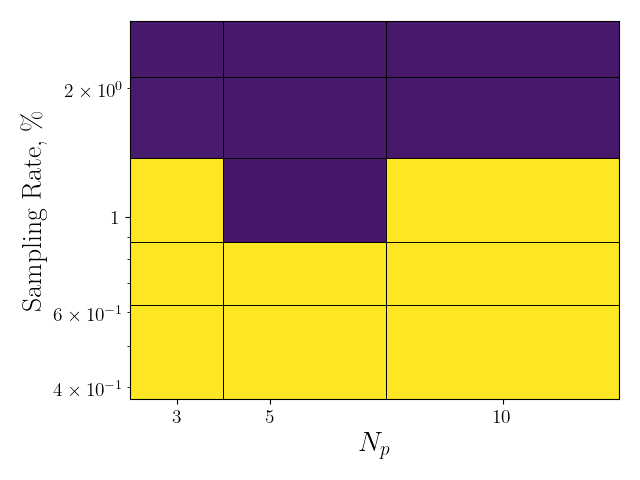
\includegraphics[width=0.99\linewidth]{Chapters/AdaptiveResults/Images/cvrc/errContours/err_contour_iter2.png}
		\subcaption{$\updateFreq = 2$}
	\end{minipage}
	\begin{minipage}{0.53\linewidth}
		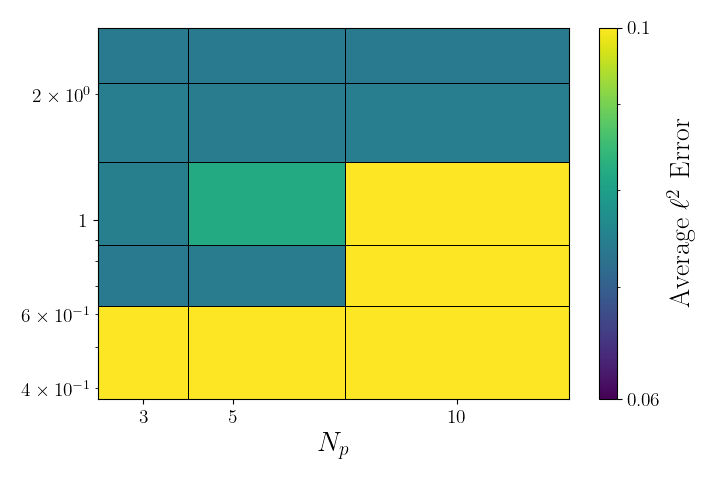
\includegraphics[width=0.99\linewidth]{Chapters/AdaptiveResults/Images/cvrc/errContours/err_contour_iter3.png}
		\subcaption{$\updateFreq = 3$}
	\end{minipage}

	\begin{minipage}{0.46\linewidth}
		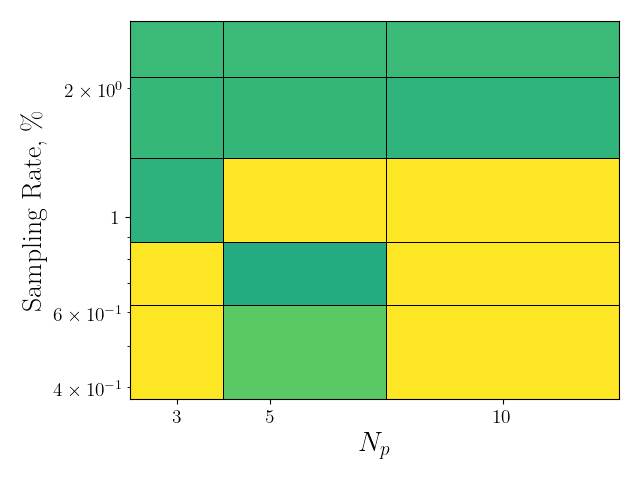
\includegraphics[width=0.99\linewidth]{Chapters/AdaptiveResults/Images/cvrc/errContours/err_contour_iter4.png}
		\subcaption{$\updateFreq = 4$}
	\end{minipage}
	\begin{minipage}{0.53\linewidth}
		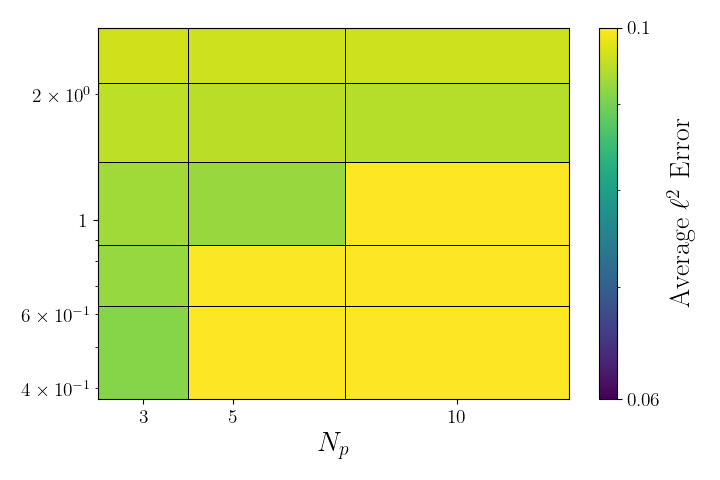
\includegraphics[width=0.99\linewidth]{Chapters/AdaptiveResults/Images/cvrc/errContours/err_contour_iter5.png}
		\subcaption{$\updateFreq = 5$}
	\end{minipage}
	\caption{\label{fig:cvrcAdaptiveROMErrContour}CVRC adaptive HPROM time-average error contours with respect to trial basis dimension and sampling rate, various $\updateFreq$.}
\end{figure}

Error contours with respect to the trial basis dimension and sampling rate, for a given update frequency, are given in Fig.~\ref{fig:cvrcAdaptiveROMErrContour}. Those cases marked in bright yellow are effectively failed simulations, incurring well in excess of 10\% error. Overall, the observed error for error stable solutions is significantly higher than that observed for the static HPROMs in Section~\ref{sec:cvrc}, ranging roughly within 6-10\%. Further, note that the tested sampling rates are much higher than those studied for the static HPROMs, and tend to require 1\% sampling to achieve stability. However, recall that the equivalent static HPROM, trained from only the first 50 $\mu$s of the FOM simulation, would invariable be unstable. Ultimately, the simulations behave similarly with respect to the sampling rate, generally improving with increased sampling. Also to be expected, accuracy tends to degrade with increased update frequency, with $\updateFreq = 5$ generating approximately $\ge 10\%$ error in all cases. Surprisingly, stability tends to decrease with respect to the trial basis dimension. This may be a function of the non-uniqueness of the one-step adaptation process, whereby a larger trial space induces a sub-optimal update. As a sanity check, the degenerative solution for $\numPrimModes = 1$ and $\primTrial^{\timeIdx} = \primVecRom^{\timeIdx}$ does not produce a stable solution.

\begin{figure}
    \begin{minipage}{0.49\linewidth}
        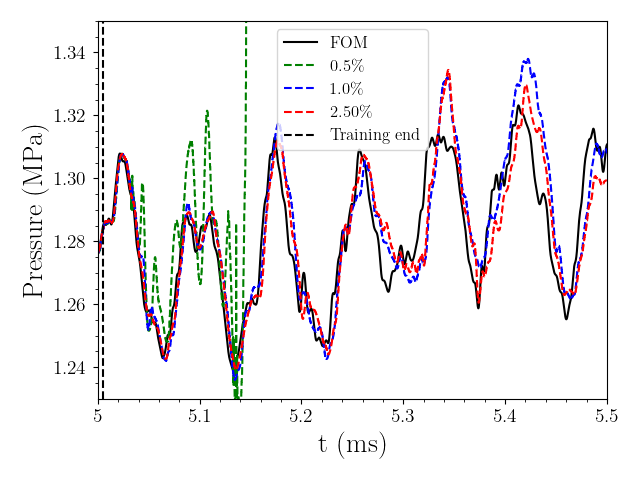
\includegraphics[width=0.99\linewidth]{Chapters/AdaptiveResults/Images/cvrc/pressure_probe_wrt_sampling.png}
        \subcaption{\label{fig:cvrcAdaptiveProbesSamps}$\updateFreq = 3$, various $\numSamps$.}
    \end{minipage}
    \begin{minipage}{0.49\linewidth}
        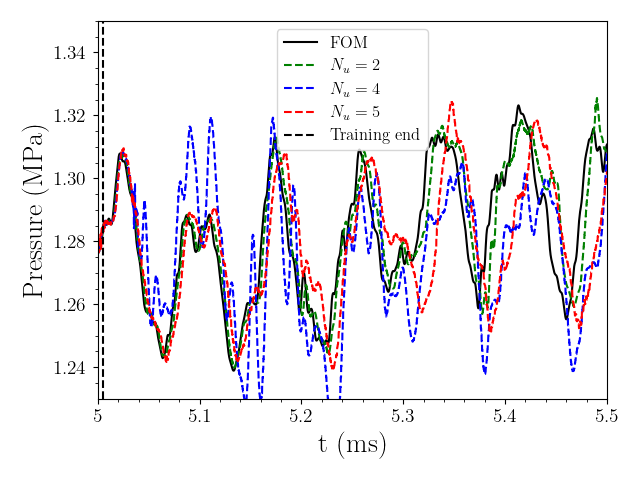
\includegraphics[width=0.99\linewidth]{Chapters/AdaptiveResults/Images/cvrc/pressure_probe_wrt_iter.png}
        \subcaption{\label{fig:cvrcAdaptiveProbesFreq}$\numSamps = 1.0\%$, various $\updateFreq$.}
    \end{minipage}
    \caption{\label{fig:cvrcAdaptiveProbes}CVRC adaptive HPROM pressure probes, $\numPrimModes = 5$.}
\end{figure}

Pressure probe monitors for several adaptive HPROM configurations are shown in Fig.~\ref{fig:cvrcAdaptiveProbes}. The end of the training period is marked by a vertical dashed line, at the far left of the images. Figure~\ref{fig:cvrcAdaptiveProbesSamps} visualizes the effect of the sampling rate on predictive performance, with the obvious conclusion that increasing the sampling rate tends to improve the pressure signal accuracy. While the case for which $\numSamps = 0.5\% \times \numDOF$ quickly becomes unstable, higher sampling rates generate near-perfect predictions up to $\timeVar = 5.3$ ms. After this point, however, significant over- and undershoots of the signal are observed, though the frequency of the dominant pressure oscillation is maintained. Figure~\ref{fig:cvrcAdaptiveProbesFreq} compares various update intervals, where previous observations are confirmed. Near-perfect prediction is achieved for $\updateFreq = 2$, while $\updateFreq = 5$ causes large discrepancies beginning at $\timeVar = 5.2$ ms and even appears to slightly decrease the frequency of the dominant acoustic mode.

\begin{figure}
	\begin{minipage}{0.99\linewidth}
		\raisebox{-0.5\height}{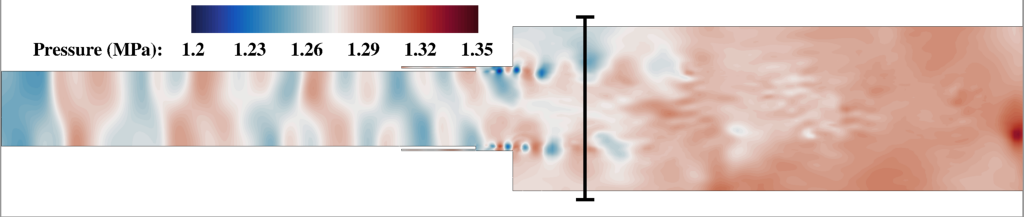
\includegraphics[width=0.84\linewidth,trim={0.5em 0.5em 0.5em 0.5em},clip]{Chapters/AdaptiveResults/Images/cvrc/fieldContours/fom_pressure_z.png}}
		\raisebox{-0.5\height}{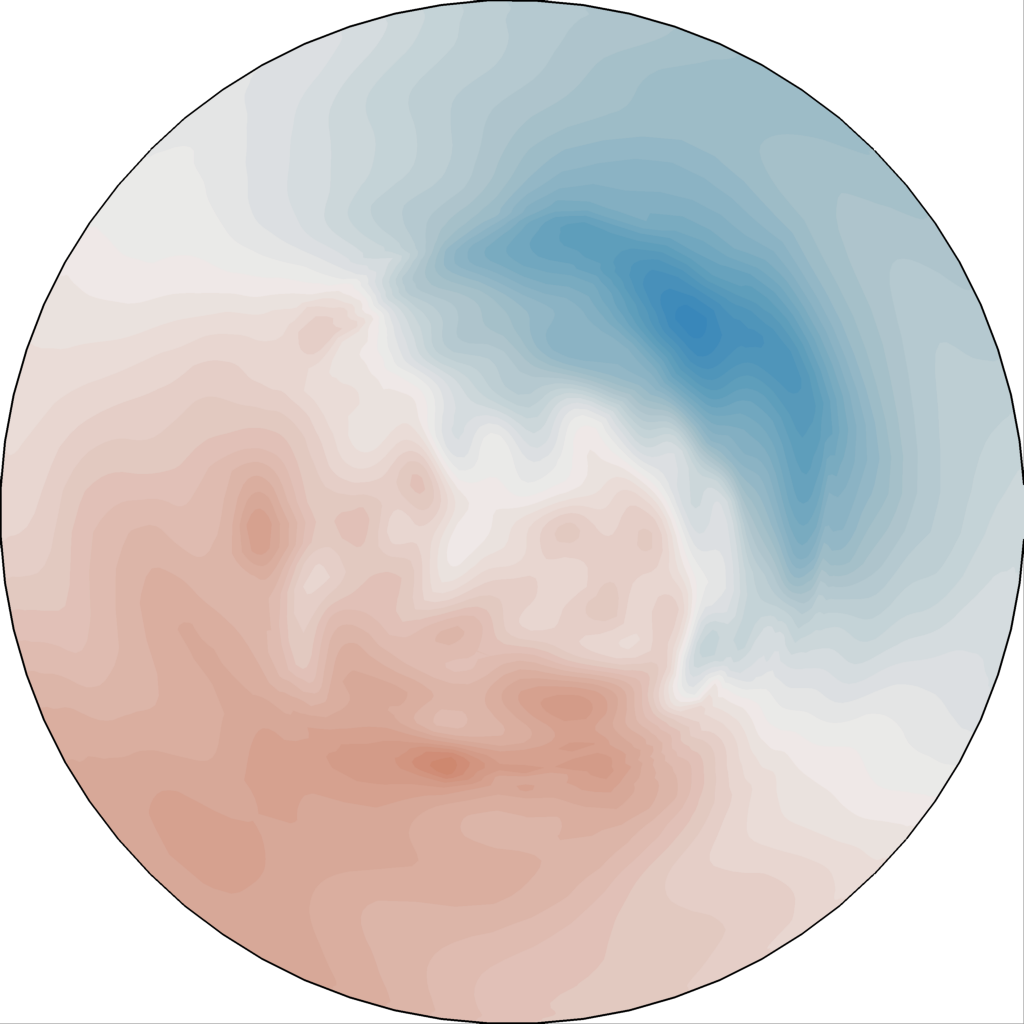
\includegraphics[width=0.14\linewidth,trim={0.0em 0.1em 0.0em 0.1em},clip]{Chapters/AdaptiveResults/Images/cvrc/fieldContours/fom_pressure_x.png}}
	\end{minipage}
    \begin{minipage}{0.99\linewidth}
		\raisebox{-0.5\height}{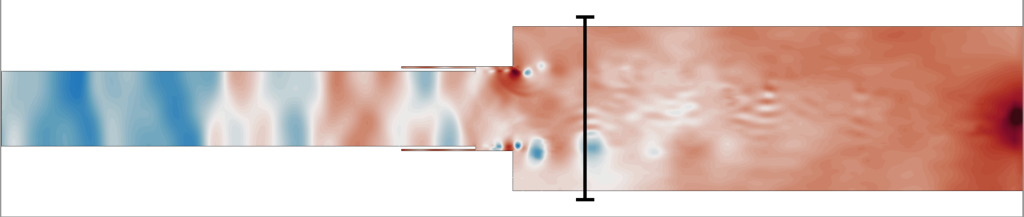
\includegraphics[width=0.84\linewidth,trim={0.5em 0.5em 0.5em 0.5em},clip]{Chapters/AdaptiveResults/Images/cvrc/fieldContours/adapt_iter2_pressure_z.png}}
		\raisebox{-0.5\height}{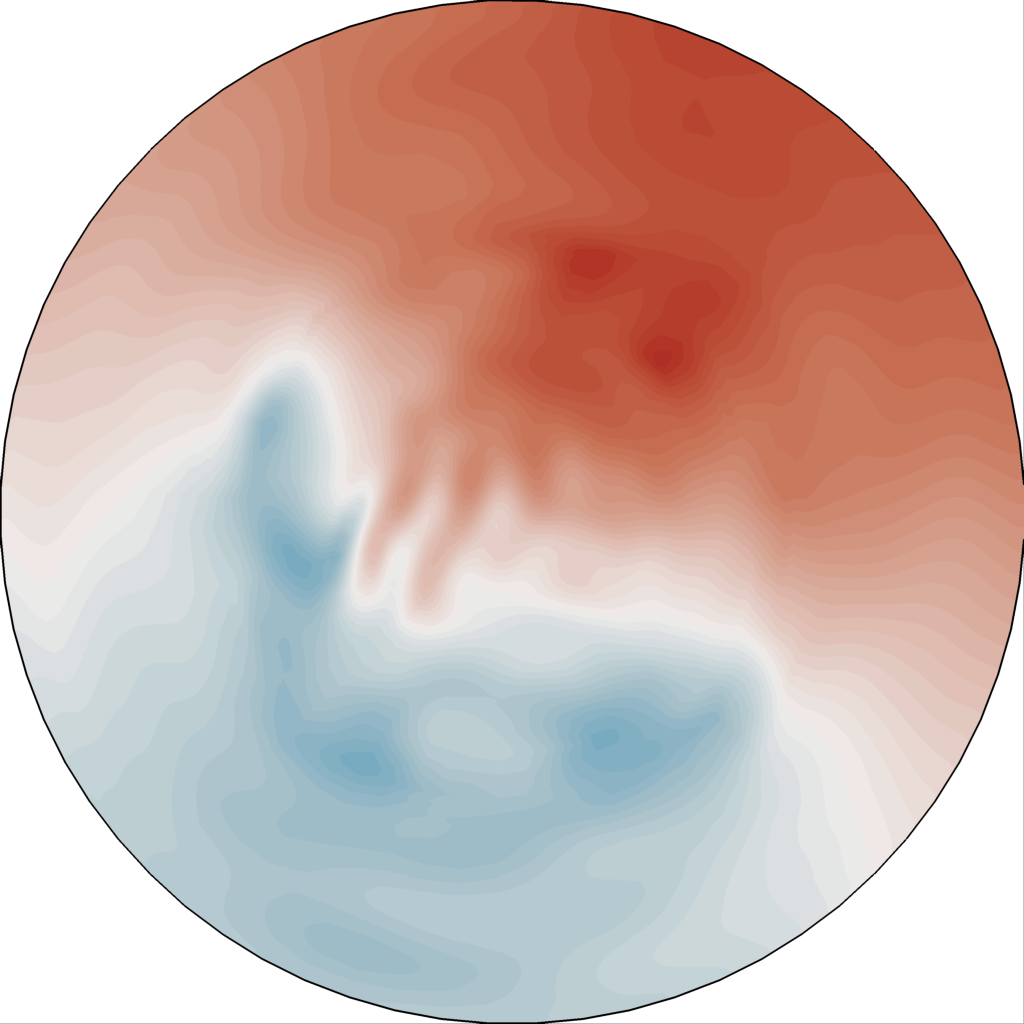
\includegraphics[width=0.14\linewidth,trim={0.0em 0.1em 0.0em 0.1em},clip]{Chapters/AdaptiveResults/Images/cvrc/fieldContours/adapt_iter2_pressure_x.png}}
	\end{minipage}
    \begin{minipage}{0.99\linewidth}
		\raisebox{-0.5\height}{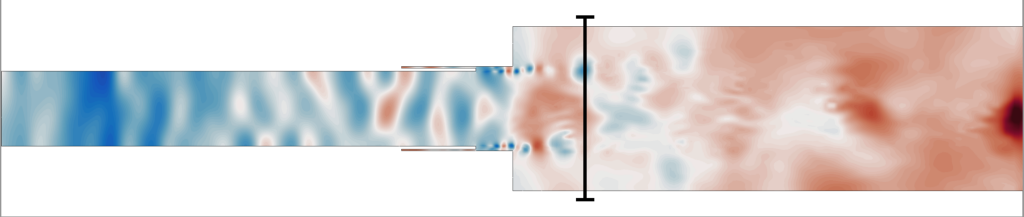
\includegraphics[width=0.84\linewidth,trim={0.5em 0.5em 0.5em 0.5em},clip]{Chapters/AdaptiveResults/Images/cvrc/fieldContours/adapt_iter4_pressure_z.png}}
		\raisebox{-0.5\height}{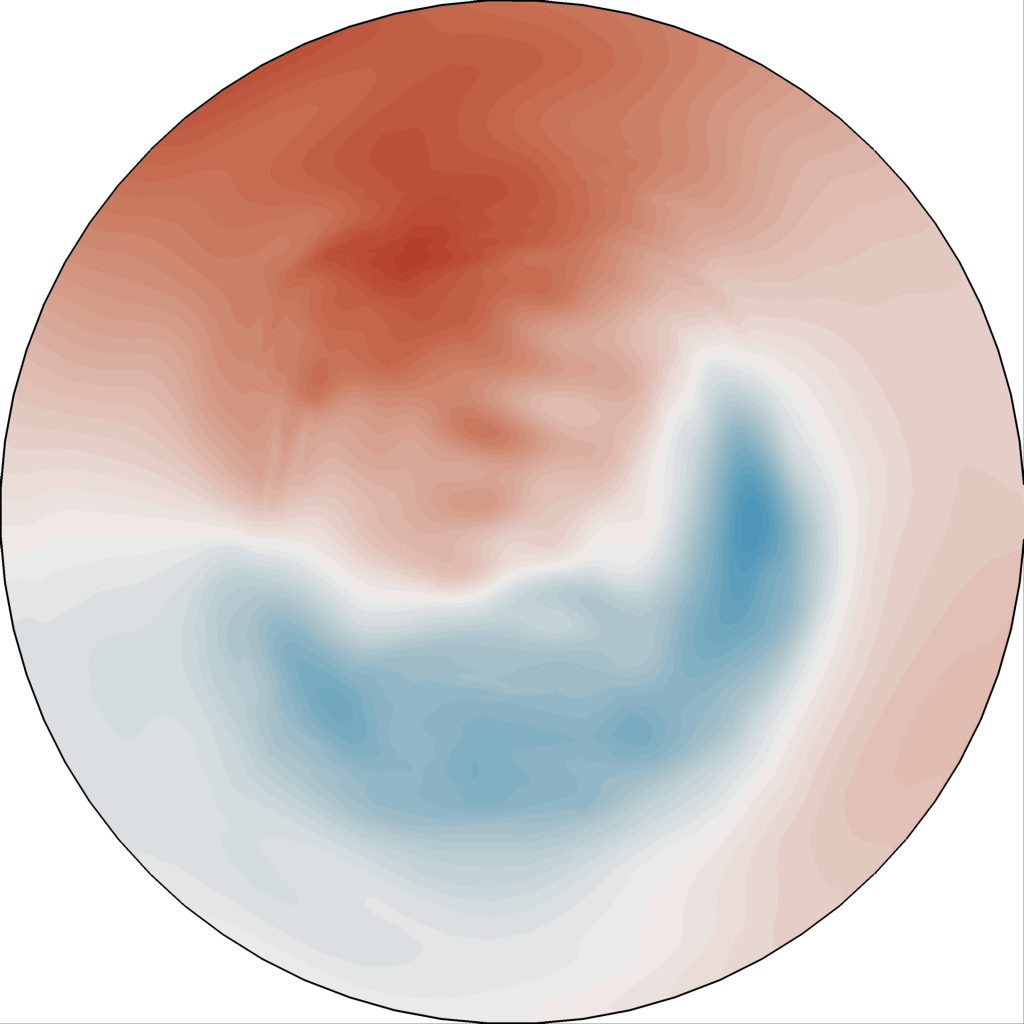
\includegraphics[width=0.14\linewidth,trim={0.0em 0.1em 0.0em 0.1em},clip]{Chapters/AdaptiveResults/Images/cvrc/fieldContours/adapt_iter4_pressure_x.png}}
	\end{minipage}
    \begin{minipage}{0.99\linewidth}
		\raisebox{-0.5\height}{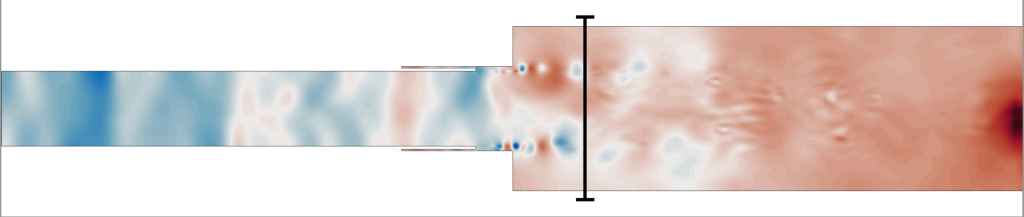
\includegraphics[width=0.84\linewidth,trim={0.5em 0.5em 0.5em 0.5em},clip]{Chapters/AdaptiveResults/Images/cvrc/fieldContours/adapt_iter5_pressure_z.png}}
		\raisebox{-0.5\height}{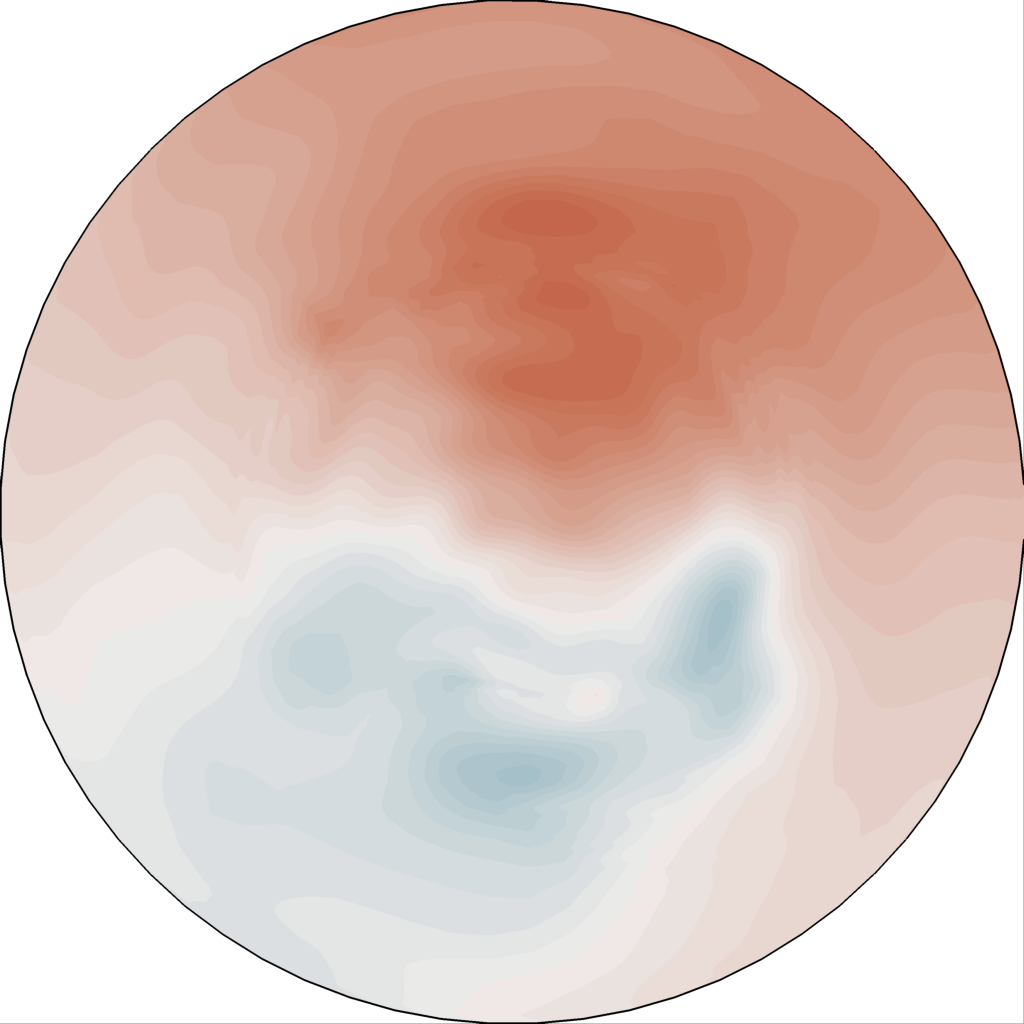
\includegraphics[width=0.14\linewidth,trim={0.0em 0.1em 0.0em 0.1em},clip]{Chapters/AdaptiveResults/Images/cvrc/fieldContours/adapt_iter5_pressure_x.png}}
	\end{minipage}
    \caption{\label{fig:cvrcAdaptiveFieldsPress}CVRC pressure field $\timeVar = 5.5$ ms, $\numPrimModes = 5$, $\numSamps = 1\% \times \numDOF$. From top to bottom: FOM, $\updateFreq = 2$, $\updateFreq = 4$, $\updateFreq = 5$.}
\end{figure}

Field comparisons at $\timeVar = 5.5$ for various update intervals are shown in Figs.~\ref{fig:cvrcAdaptiveFieldsPress} and~\ref{fig:cvrcAdaptiveFieldsTemp}. Although relative accuracy is not immediately obvious, in the pressure fields shown in Fig.~\ref{fig:cvrcAdaptiveFieldsPress} it is apparent that the highly-inaccurate case for $\updateFreq = 4$ gives rise to spurious high-frequency oscillations along the center axis of the combustion chamber, just downstream of the dump plane. The evolution of the temperature field in Fig.~\ref{fig:cvrcAdaptiveFieldsTemp} is similarly opaque, though all appear to generate the characteristic shear layer and vigorous mixing near the exit.

\begin{figure}
	\begin{minipage}{0.99\linewidth}
		\raisebox{-0.5\height}{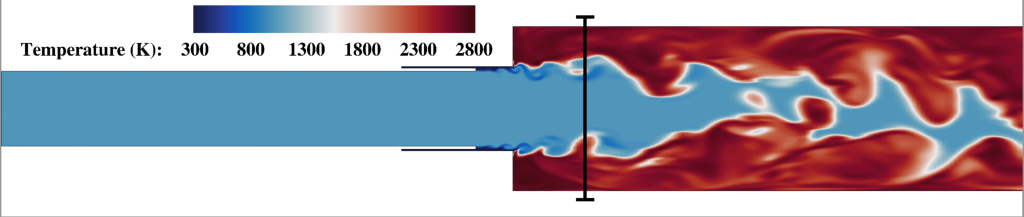
\includegraphics[width=0.84\linewidth,trim={0.5em 0.5em 0.5em 0.5em},clip]{Chapters/AdaptiveResults/Images/cvrc/fieldContours/fom_temperature_z.png}}
		\raisebox{-0.5\height}{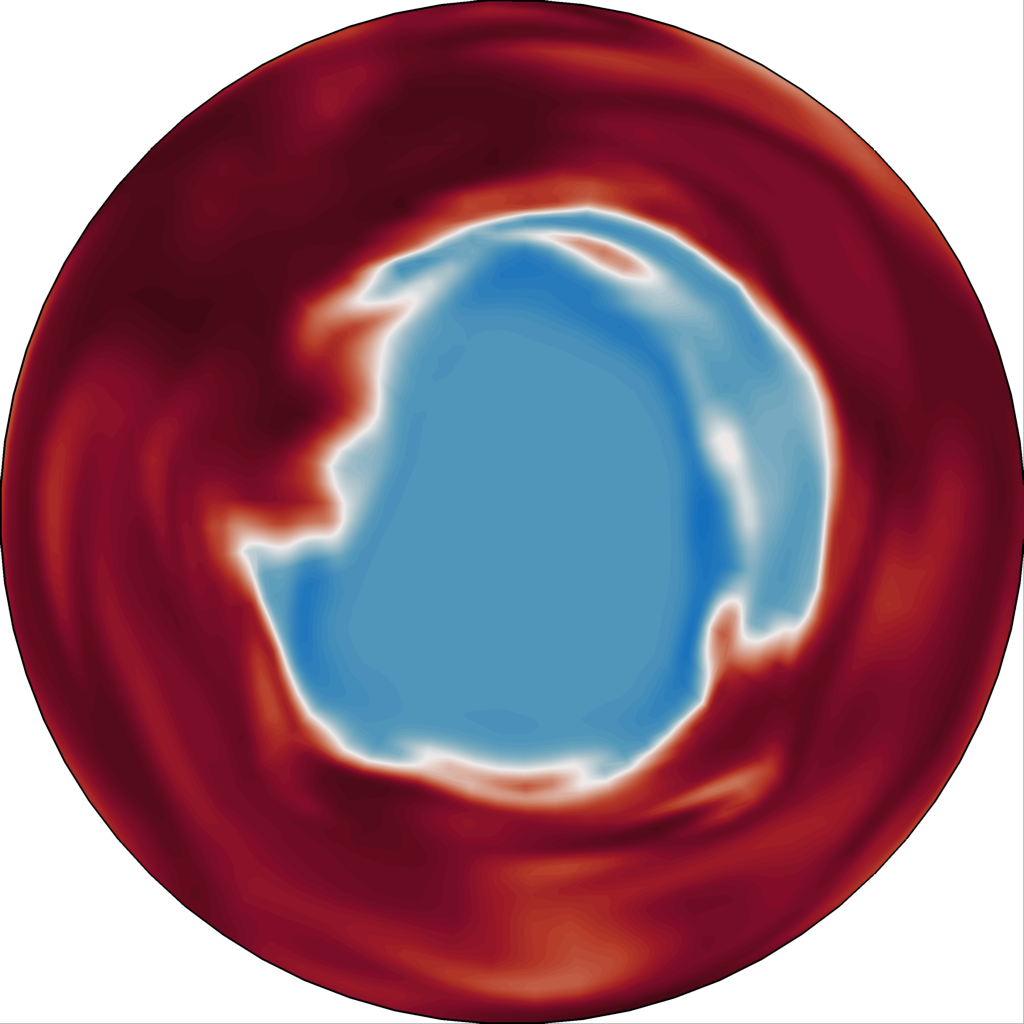
\includegraphics[width=0.14\linewidth,trim={0.0em 0.1em 0.0em 0.1em},clip]{Chapters/AdaptiveResults/Images/cvrc/fieldContours/fom_temperature_x.png}}
	\end{minipage}
    \begin{minipage}{0.99\linewidth}
		\raisebox{-0.5\height}{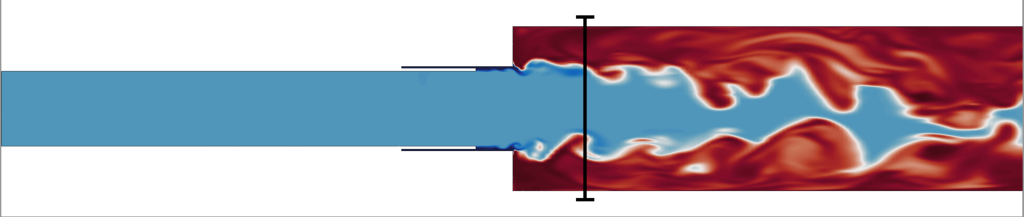
\includegraphics[width=0.84\linewidth,trim={0.5em 0.5em 0.5em 0.5em},clip]{Chapters/AdaptiveResults/Images/cvrc/fieldContours/adapt_iter2_temperature_z.png}}
		\raisebox{-0.5\height}{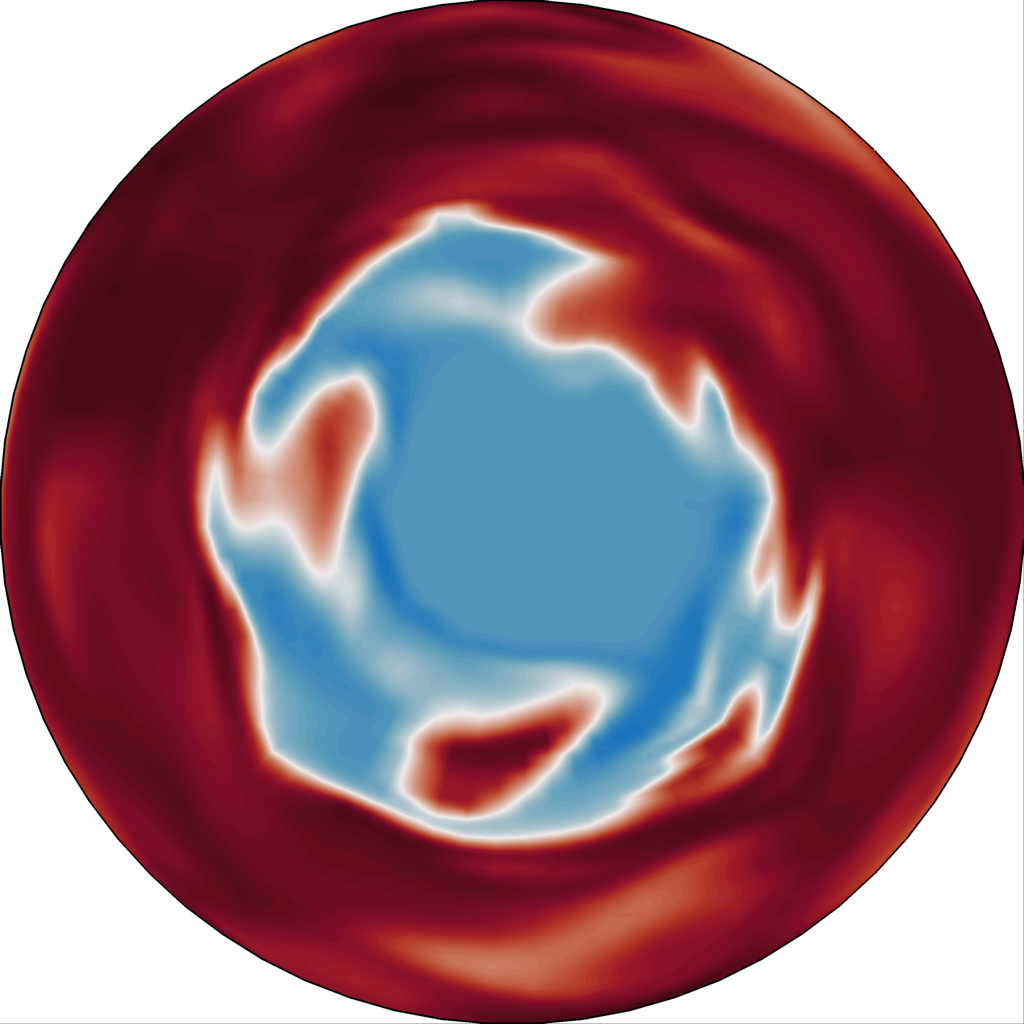
\includegraphics[width=0.14\linewidth,trim={0.0em 0.1em 0.0em 0.1em},clip]{Chapters/AdaptiveResults/Images/cvrc/fieldContours/adapt_iter2_temperature_x.png}}
	\end{minipage}
    \begin{minipage}{0.99\linewidth}
		\raisebox{-0.5\height}{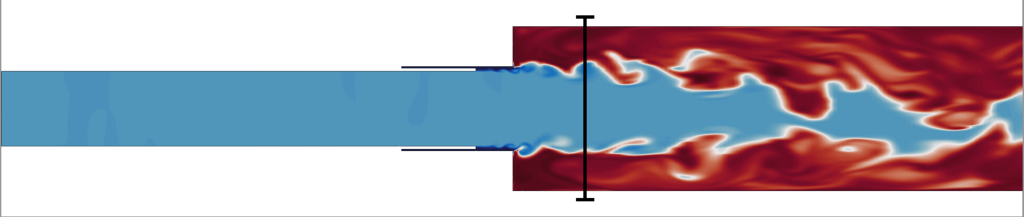
\includegraphics[width=0.84\linewidth,trim={0.5em 0.5em 0.5em 0.5em},clip]{Chapters/AdaptiveResults/Images/cvrc/fieldContours/adapt_iter4_temperature_z.png}}
		\raisebox{-0.5\height}{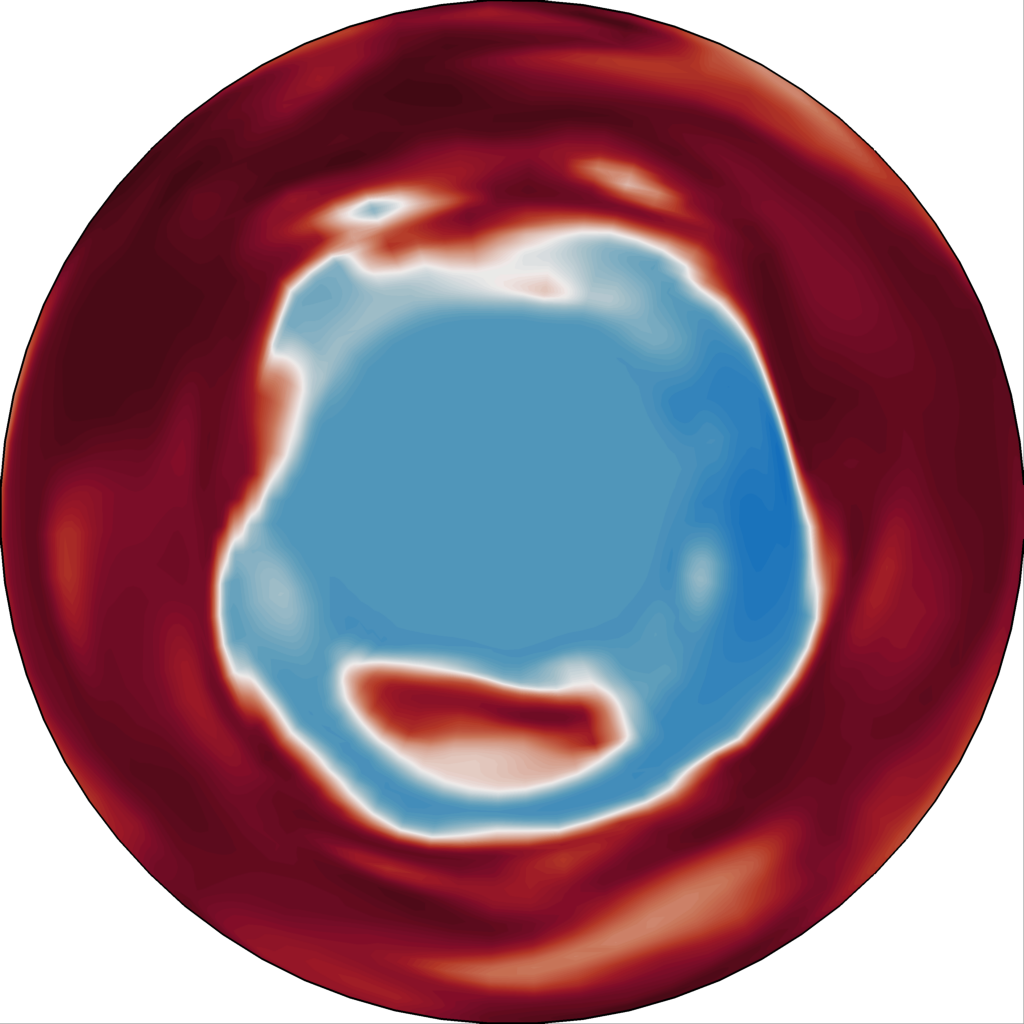
\includegraphics[width=0.14\linewidth,trim={0.0em 0.1em 0.0em 0.1em},clip]{Chapters/AdaptiveResults/Images/cvrc/fieldContours/adapt_iter4_temperature_x.png}}
	\end{minipage}
    \begin{minipage}{0.99\linewidth}
		\raisebox{-0.5\height}{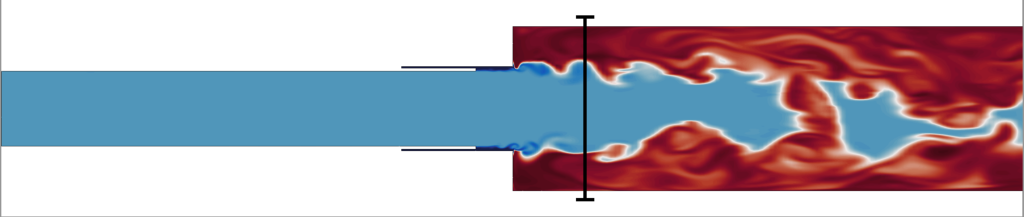
\includegraphics[width=0.84\linewidth,trim={0.5em 0.5em 0.5em 0.5em},clip]{Chapters/AdaptiveResults/Images/cvrc/fieldContours/adapt_iter5_temperature_z.png}}
		\raisebox{-0.5\height}{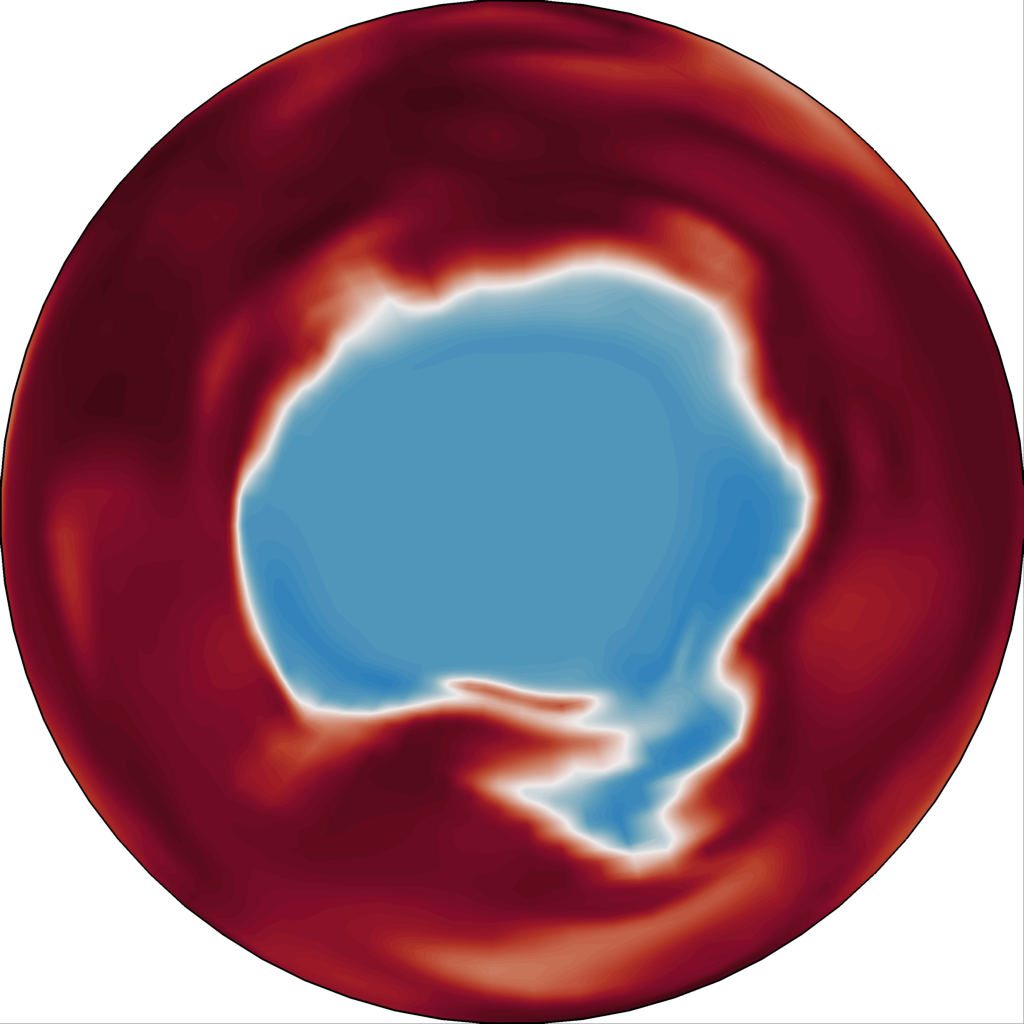
\includegraphics[width=0.14\linewidth,trim={0.0em 0.1em 0.0em 0.1em},clip]{Chapters/AdaptiveResults/Images/cvrc/fieldContours/adapt_iter5_temperature_x.png}}
	\end{minipage}
    \caption{\label{fig:cvrcAdaptiveFieldsTemp}CVRC temperature field $\timeVar = 5.5$ ms, $\numPrimModes = 5$, $\numSamps = 1\% \times \numDOF$. From top to bottom: FOM, $\updateFreq = 2$, $\updateFreq = 4$, $\updateFreq = 5$.}
\end{figure}

The process of sample mesh adaptation is briefly touched upon. Recall that the error metric used to select a new sample set is computed from the regression error of the full field $\primVecRom$. This metric is computed in one shot, and does not involve any greedy iteration process like those outlined in Section~\ref{subsec:sampAlgos}. As such, the sample mesh slices shown in Fig.~\ref{fig:cvrcAdaptiveIBlankSlice} are largely unsurpising, generating extremely tight clusters of samples similar to those generated by GNAT sampling as seen in Section~\ref{sec:cvrc}. Again, samples tend to be selected in the reacting shear layer, which is characterized by highly unsteady mixing and sharp gradients at the flame front. Isosurfaces of the directly-sampled mesh elements in Fig.~\ref{fig:cvrcAdaptiveIBlankIso} emphasize this, generating a nearly conical sample mesh similar to those observed for eigenvector-based sampling in Section~\ref{sec:cvrc}.

\begin{figure}
	\begin{minipage}{0.99\linewidth}
		\raisebox{-0.5\height}{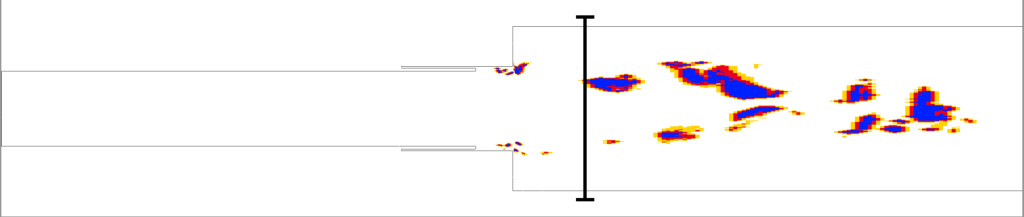
\includegraphics[width=0.84\linewidth,trim={0.5em 0.5em 0.5em 0.5em},clip]{Chapters/AdaptiveResults/Images/cvrc/iblank/iblank_z_1025.png}}
		\raisebox{-0.5\height}{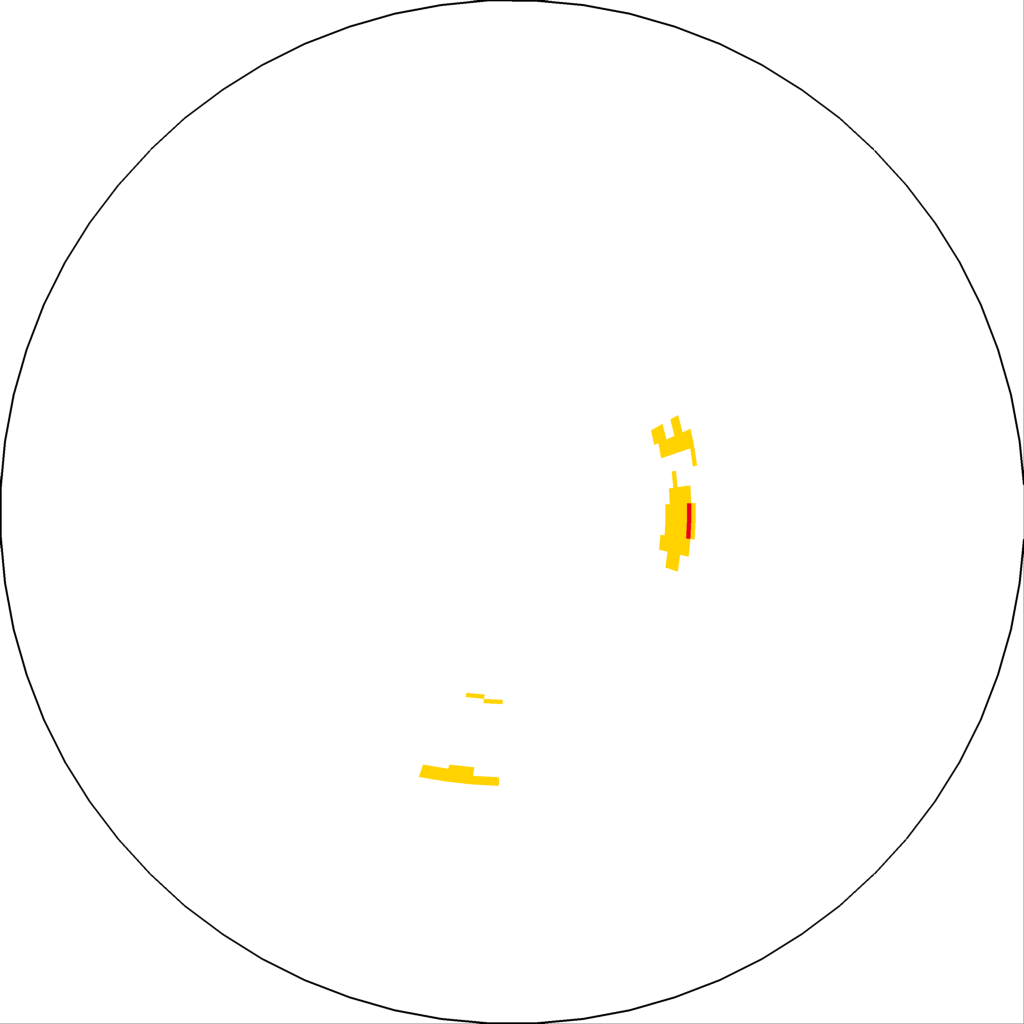
\includegraphics[width=0.14\linewidth,trim={0.0em 0.1em 0.0em 0.1em},clip]{Chapters/AdaptiveResults/Images/cvrc/iblank/iblank_x_1025.png}}
	\end{minipage}
    \begin{minipage}{0.99\linewidth}
		\raisebox{-0.5\height}{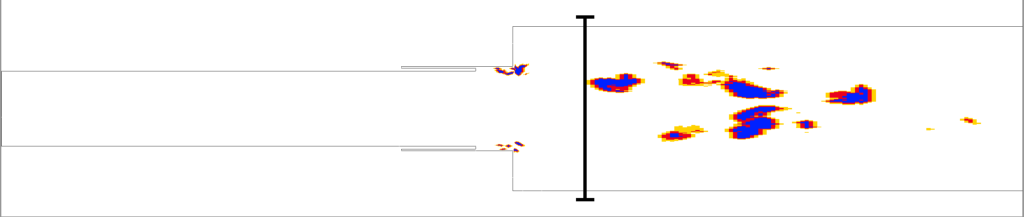
\includegraphics[width=0.84\linewidth,trim={0.5em 0.5em 0.5em 0.5em},clip]{Chapters/AdaptiveResults/Images/cvrc/iblank/iblank_z_1050.png}}
		\raisebox{-0.5\height}{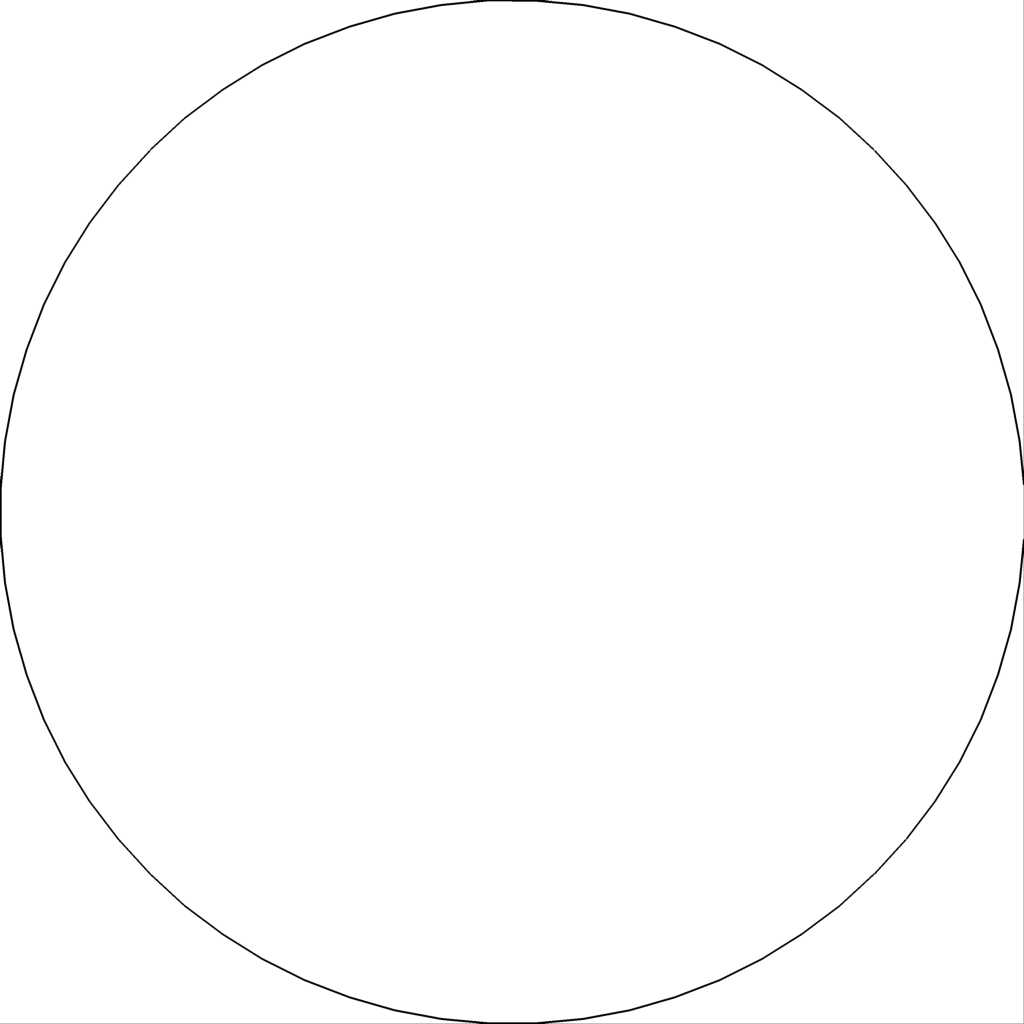
\includegraphics[width=0.14\linewidth,trim={0.0em 0.1em 0.0em 0.1em},clip]{Chapters/AdaptiveResults/Images/cvrc/iblank/iblank_x_1050.png}}
	\end{minipage}
    \begin{minipage}{0.99\linewidth}
		\raisebox{-0.5\height}{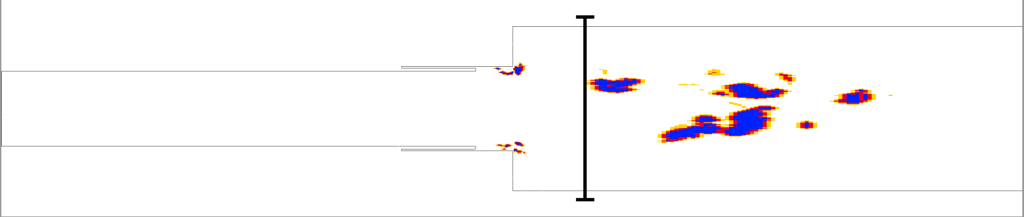
\includegraphics[width=0.84\linewidth,trim={0.5em 0.5em 0.5em 0.5em},clip]{Chapters/AdaptiveResults/Images/cvrc/iblank/iblank_z_1075.png}}
		\raisebox{-0.5\height}{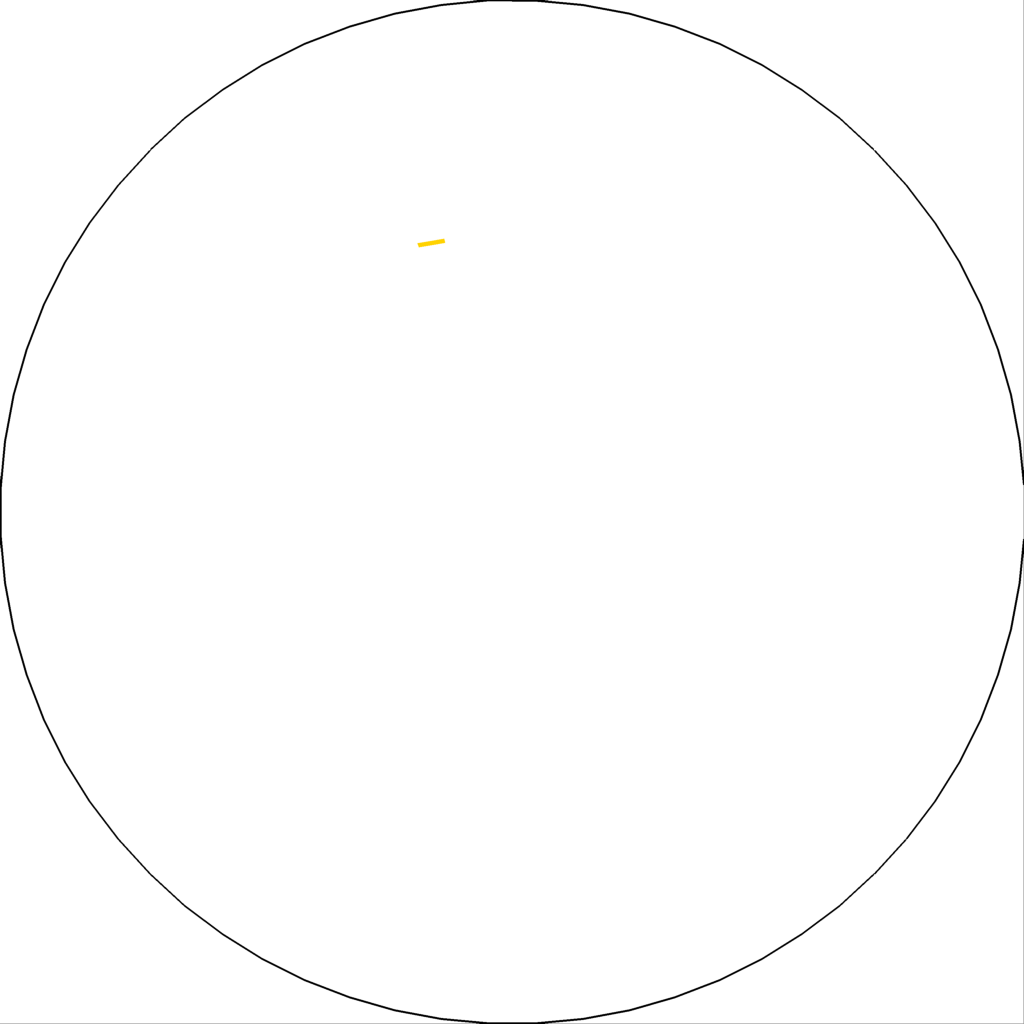
\includegraphics[width=0.14\linewidth,trim={0.0em 0.1em 0.0em 0.1em},clip]{Chapters/AdaptiveResults/Images/cvrc/iblank/iblank_x_1075.png}}
	\end{minipage}
    \begin{minipage}{0.99\linewidth}
		\raisebox{-0.5\height}{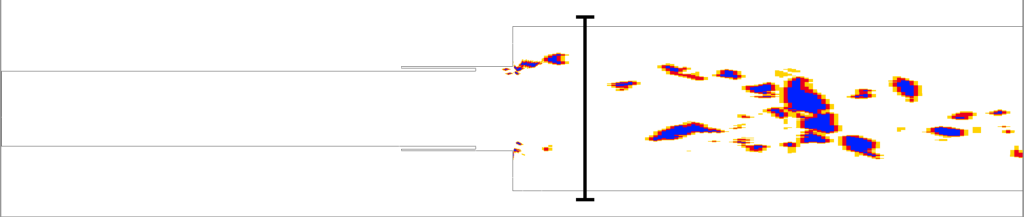
\includegraphics[width=0.84\linewidth,trim={0.5em 0.5em 0.5em 0.5em},clip]{Chapters/AdaptiveResults/Images/cvrc/iblank/iblank_z_1100.png}}
		\raisebox{-0.5\height}{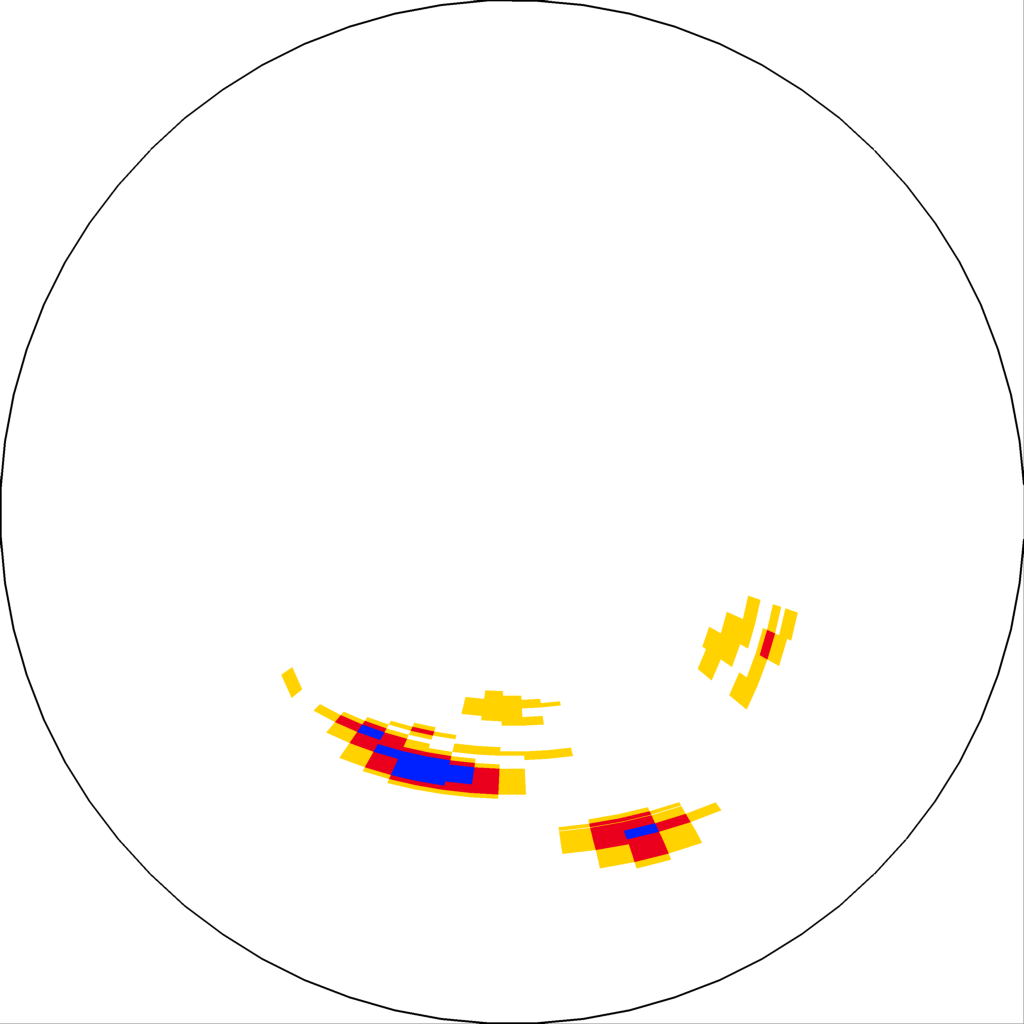
\includegraphics[width=0.14\linewidth,trim={0.0em 0.1em 0.0em 0.1em},clip]{Chapters/AdaptiveResults/Images/cvrc/iblank/iblank_x_1100.png}}
	\end{minipage}
    \caption{\label{fig:cvrcAdaptiveIBlankSlice}CVRC sample mesh, $\numPrimModes = 5$, $\numSamps = 1\% \times \numDOF$. From top to bottom, $\timeVar = 5.125$ ms, $5.25$ ms, $5.375$ ms, $5.5$ ms.}
\end{figure}

\begin{figure}
	\centering
	\begin{minipage}{0.45\linewidth}
		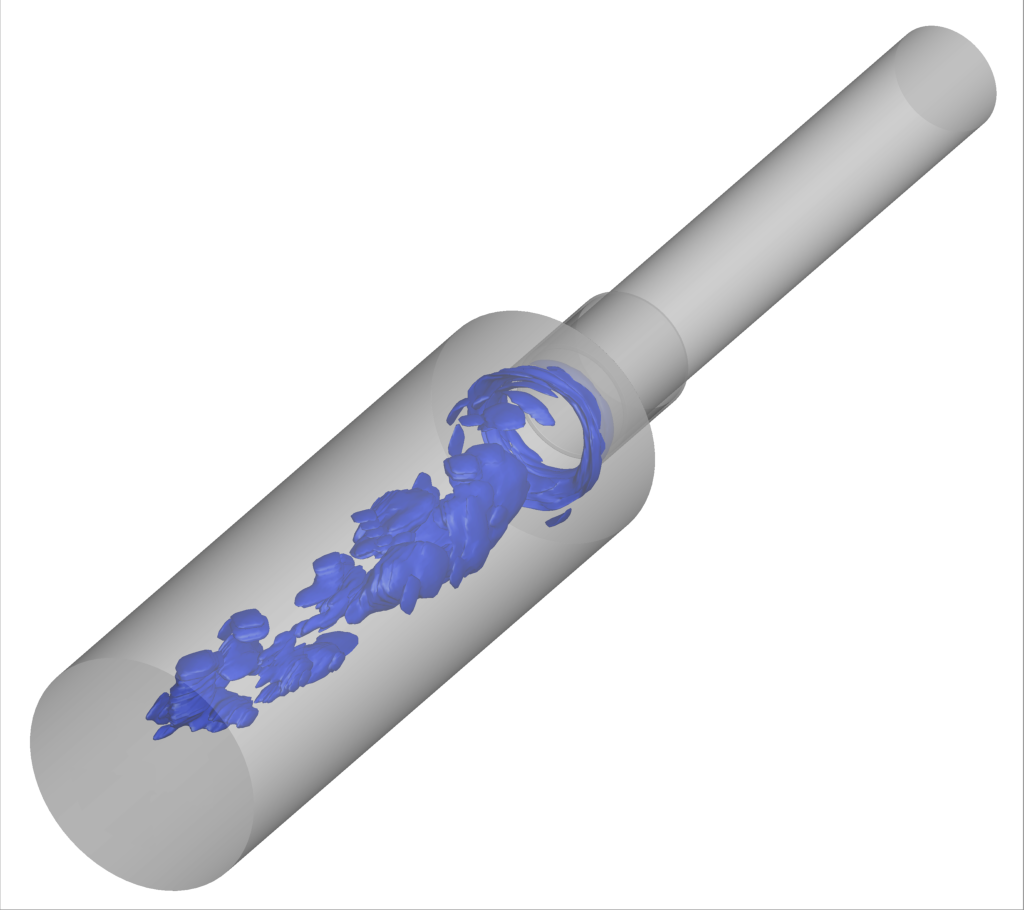
\includegraphics[width=0.99\linewidth,trim={0.5em 0.5em 0.5em 0.5em},clip]{Chapters/AdaptiveResults/Images/cvrc/iblank/iblank_iso_1025.png}
	\end{minipage}
	\begin{minipage}{0.45\linewidth}
		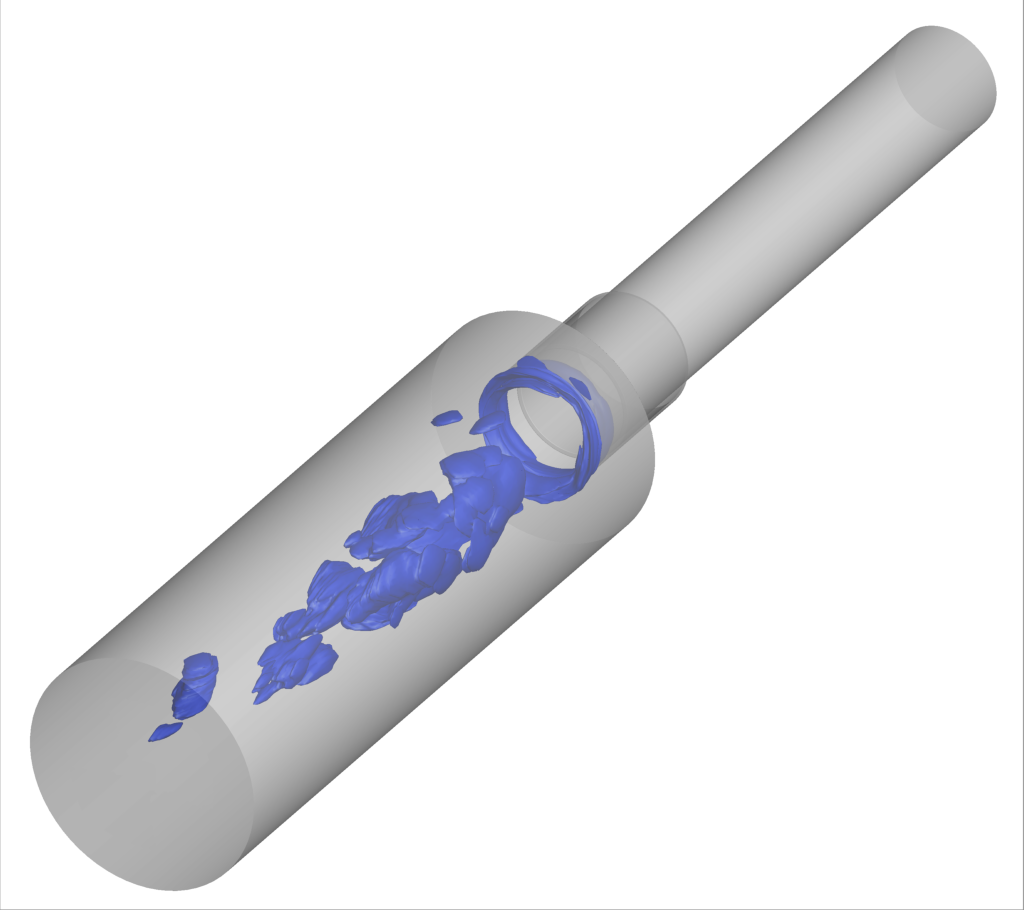
\includegraphics[width=0.99\linewidth,trim={0.5em 0.5em 0.5em 0.5em},clip]{Chapters/AdaptiveResults/Images/cvrc/iblank/iblank_iso_1050.png}
	\end{minipage}

	\centering
	\begin{minipage}{0.45\linewidth}
		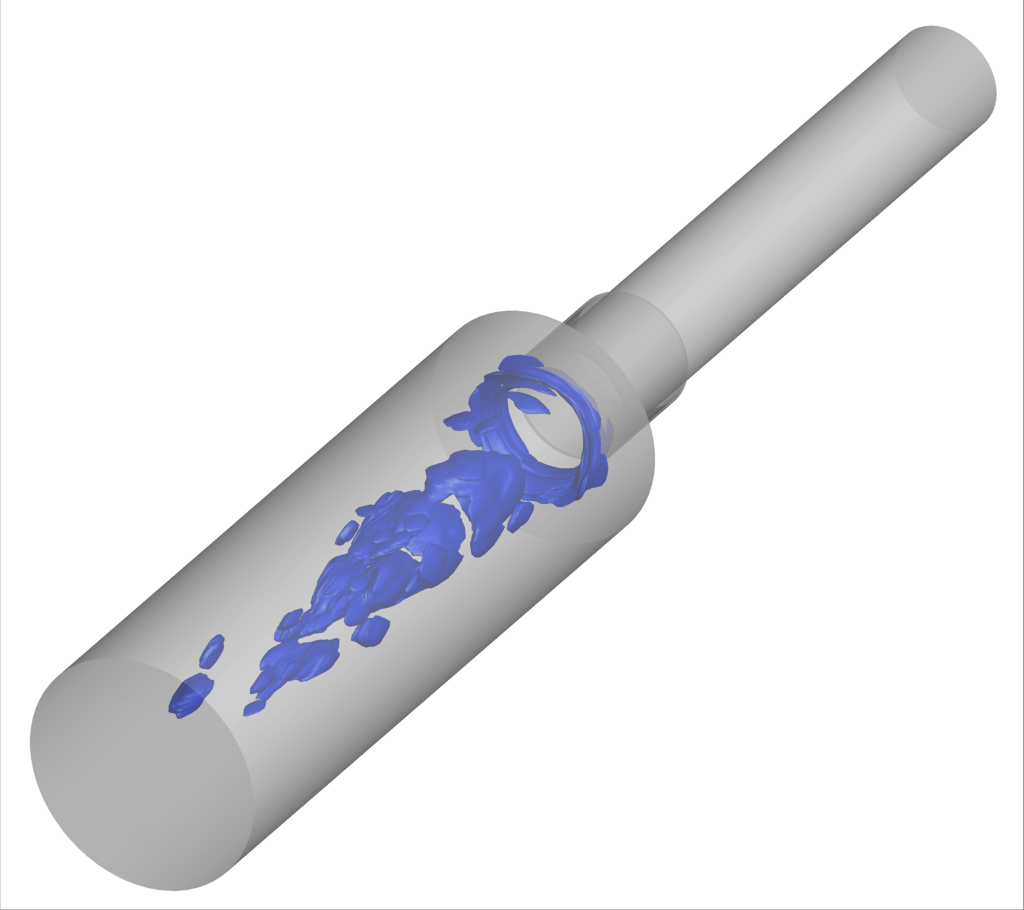
\includegraphics[width=0.99\linewidth,trim={0.5em 0.5em 0.5em 0.5em},clip]{Chapters/AdaptiveResults/Images/cvrc/iblank/iblank_iso_1075.png}
	\end{minipage}
	\begin{minipage}{0.45\linewidth}
		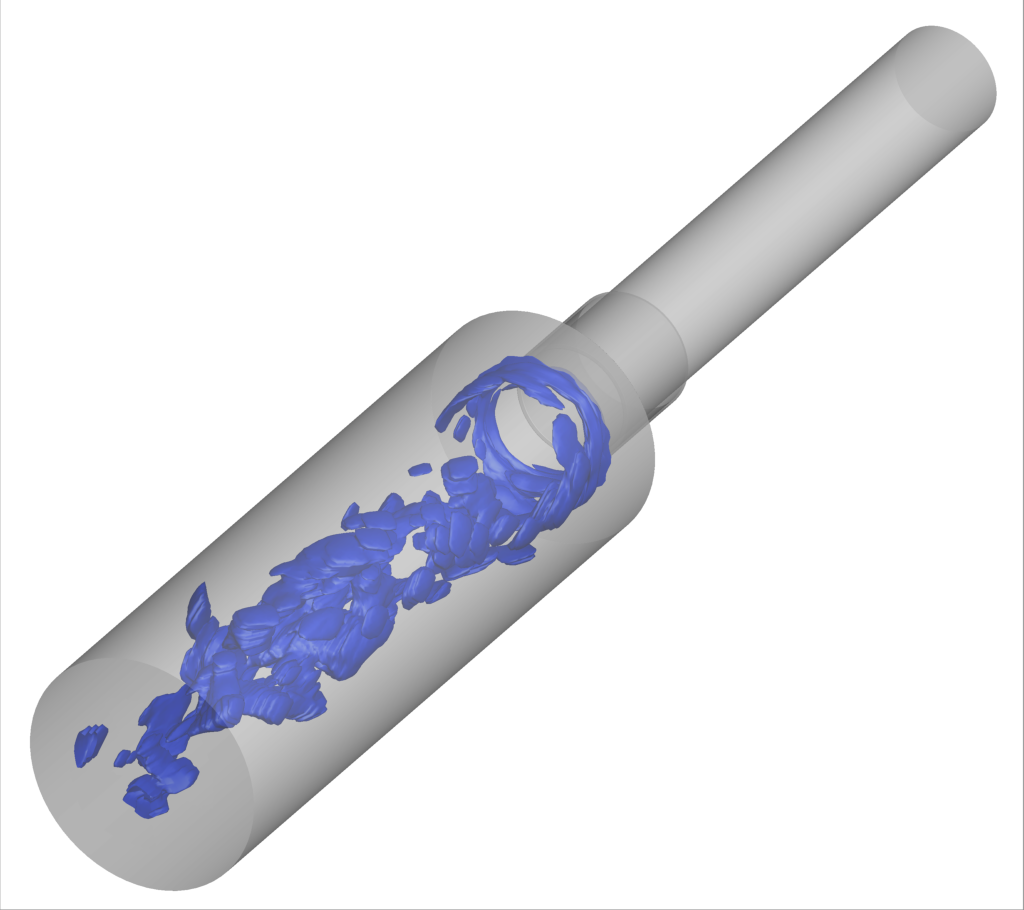
\includegraphics[width=0.99\linewidth,trim={0.5em 0.5em 0.5em 0.5em},clip]{Chapters/AdaptiveResults/Images/cvrc/iblank/iblank_iso_1100.png}
	\end{minipage}
	\caption{\label{fig:cvrcAdaptiveIBlankIso}Directly-sampled cell isosurfaces, $\numPrimModes = 5$, $\numSamps = 1\% \times \numDOF$. Top left is $\timeVar = 5.125$ ms, top right is $5.25$ ms, bottom left is $5.375$ ms, bottom right is $5.5$ ms.}
\end{figure}

Although the predictive performance of these adaptive HPROMs shown above are quite remarkable, they are not without major drawbacks. Primary among those for the adaptive approach used here is the need to compute the full-order solution at the interval specified by $\updateFreq$. For the cases explored here, for which half of the subiterations for an adaptation step are dedicated to the FOM solve, the absolute maximum computational speedup that can be achieved is thus equal to $2 \times \updateFreq$. This is confirmed in Fig.~\ref{fig:cvrcAdaptivePareto}, which displays the tradeoff in error with respect to computational speedup for all HPROMs computed. Each line represents one value of $\updateFreq$, and each point represents a different sampling rate. Although these results indicate that the solver is able to nearly achieve the upper bound of computational speedup, the cost savings are paltry compared to those observed for the static HPROMs in Chapter~\ref{chap:HPROMResults}. Further, the sampling rate appears to have little effect on the overall accuracy or computational speedup beyond a certain point, as any speedup is inevitably dwarfed by the cost of the sampling update step.

\begin{figure}
    \centering
    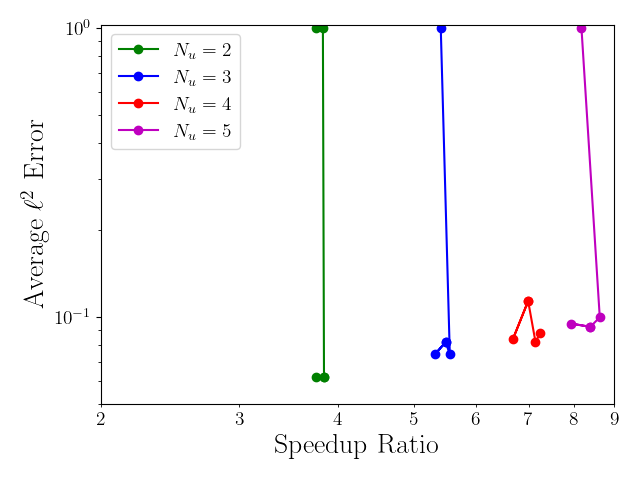
\includegraphics[width=0.5\linewidth]{Chapters/AdaptiveResults/Images/cvrc/pareto_wrt_iters_Average_errorRaw_pareto.png}
    \caption{\label{fig:cvrcAdaptivePareto}CVRC adaptive HPROM time-average error vs. computational speedup, $\numPrimModes = 5$, various $\updateFreq$.}
\end{figure}